\section{Mental Factors (\textit{Cetasika})}

Welcome to the fourth talk of this Practical Abhidhamma Course.\footnote{More details in Chapter 2 of “A Comprehensive Manual of Abhidhamma” and “Cetasikas” (see Footnote 2).} This talk will describe Mental Factors, the second of the four Ultimate Realities (\textit{citta}, \textit{cetasika}, \textit{rūpa} and \textit{Nibbāna}). For this talk, you should have the \textit{Satipaṭṭhāna} Sutta printout, Handout 2, Handout 3 and Handout 4 in front of you.

Handout 3 is like a glossary for the 52 Mental Factors. The words being defined are in the first column. These include “\textbf{Contact},” “\textbf{Feeling},” “\textbf{Perception}” all the way to “\textbf{Abstinence from wrong livelihood}.” The remaining columns, “Pāḷi,” “Characteristic,” “Function,” “Manifestation” and “Proximate Cause” give more information on the word being defined.

There is rarely a perfect fit when translating a word from one language to another. For example, when I use the word “\textbf{Contact}” during my talks, or when you read the word “\textbf{Contact}” in a Sutta translation, the actual meaning is a combination of the English words “contact” and “sense impression.” If you think back to our discussion of “\textbf{Feeling}” in the last talk, you can see how this Mental Factor has a meaning that combines “feeling,” “sensation” and “experience.”

I would like to share an analogy. We can say that a company includes management, sales and finance. One perspective is that management, sales and finance are titles or people; in other words, a company is a collection of nouns. Another perspective is that management, sales and finance are interdependent activities; in other words, a company is a collection of verbs. Each perspective provides a different insight into the nature of the thing called a company.

One perspective is that consciousness and the Mental Factors are nouns; components of a Thought Moment. Another perspective is that consciousness and the Mental Factors are verbs; interdependent activities within a Thought Moment. Each perspective provides a different insight into the nature of the thing called a Thought Moment.

As we go through Mental Factors in this talk, you may first want to think of them as components of a Thought Moment, and then think of them again as interdependent activities to get a different perspective.

Just because all Mental Factors within a Thought Moment are interdependent and function as a team, does not imply that they are all equal. Reflect upon your own experience of a Thought Moment in the Danger Zone or in the Faultless Zone; is it not apparent that the roots of \textbf{Attachment}, \textbf{Aversion}, \textbf{Delusion}, \textbf{Non-attachment}, \textbf{Non-aversion} and \textbf{Understanding}, tend to dominate everything in the Thought Moment,\footnote{In the \textit{Paṭṭhāna}, this is called “Root condition” (\textit{hetu-paccaya}). More details in Chapter 2 of “The Conditionality of Life” (see Footnote 2).} and extend their influence to speech and actions?\footnote{“Speech and actions” means the mind-born groups of \textit{rūpas} with \textbf{Bodily-indication}/\textbf{Verbal-indication}.}

I will not use Pāḷi words from Handout 3 in this talk. If you want to start learning a bit of Pāḷi, the names of the Mental Factors are a good starting point because these are very important words in the Suttas.

The Commentary provides a very structured definition for each Mental Factor. It looks at each Mental Factor from four angles: the characteristic is the main quality of this Mental Factor; the function defines the role that this Mental Factor plays, or the goal that this Mental Factor achieves in the Thought Moment; the manifestation describes how this Mental Factor is experienced during meditation, and the proximate cause explains the main thing that typically causes this Mental Factor to come into prominence.

\pagebreak

I suggest that while I am talking about a Mental Factor, you quickly scan the other columns to get a fuller picture of what is meant by that Mental Factor. If something is confusing, ignore it; don’t let it slow you down. You can always go back later and read the footnotes in the document if needed. The details in the other columns are not that important for a beginner.

\begin{figure}[h]
\centering

\includegraphics[width=1.0\linewidth]{./Diagrams/Ment_Fact}
\caption{{\small \textit{The types of Mental Factors that arise in each Thought Moment will depend on the type of Thought Moment }(Unwholesome/Rootless/Wholesome).}}
\label{fig:MentalFactors}
\end{figure}

Now, let’s take a look at how this list of Mental Factors is organized in Handout 3. There are three groups of Mental Factors, numbered 1, 2 and 3.

The first group of Mental Factors are ethically-variable. This is group 1 starting with “\textbf{Contact}.” When ethically-variable Mental Factors arise in unwholesome Thought Moments, they are unwholesome. When ethically-variable Mental Factors arise in ethically-neutral Thought Moments, they are neutral. When ethically-variable Mental Factors arise in wholesome Thought Moments, they are wholesome.

The second group of Mental Factors are unwholesome. This is group 2 starting with “\textbf{Delusion}.” Unwholesome Mental Factors arise only in unwholesome Thought Moments.

The third group of Mental Factors are beautiful. This is group 3 starting with “\textbf{Faith}.” Beautiful Mental Factors arise only in wholesome Thought Moments.

Within each of the three groups of Mental Factors are two subgroups; universals and occasionals. The universal ethically-variable Mental Factors are the seven starting with “\textbf{Contact}.” The occasional ethically-variable Mental Factors are the six starting with “\textbf{Initial application}.” The universal unwholesome Mental Factors are the four starting with “\textbf{Delusion}.” The occasional unwholesome Mental Factors are the 10 starting with “\textbf{Attachment}.” The universal beautiful Mental Factors are the nineteen starting with “\textbf{Faith}” (some of the Mental Factors are counted twice to get a total of 19). The occasional beautiful Mental Factors are the six starting with “\textbf{Understanding}.”

Handout 4 combines information from Handout 2 and from Handout 3. Handout 4 shows which Mental Factors are included in each Thought Moment. The rows in Handout 4 are numbered \textbf{1}--\textbf{81}, corresponding to the numbering of the Thought Moments in Handout 2. The Supramundane Thought Moments, Thought Moments \textbf{82}--\textbf{89}, can get a bit complicated, so they are not included in Handout 4. The columns in Handout 4 correspond to the list of Mental Factors in Handout 3. A grey square indicates that this Mental Factor arises in this Thought Moment. No grey square indicates that this Mental Factor does not arise in this Thought Moment. A grey triangle indicates that this Mental Factor sometimes arises in this Thought Moment and sometimes does not arise in this Thought Moment.

Let us go through two examples to show how to use Handout 4. According to Handout 2, Thought Moment \textbf{1} is unwholesome, \textbf{Attachment}-rooted, unprompted, associated with \textbf{Wrong view} and accompanied by pleasant \textbf{Feeling}. If we look at Handout 4, we can see that Thought Moment \textbf{1} includes all seven of the universal ethically-variable Mental Factors, all six of the occasional ethically-variable Mental Factors, all four of the universal unwholesome Mental Factors, and \textbf{Attachment} and \textbf{Wrong view}.

For our second example, let us consider the six roots that are the foundation of Buddhist ethics. As I mentioned in the previous talk, the three unwholesome roots are \textbf{Attachment}, \textbf{Aversion} and \textbf{Delusion}, and the three beautiful roots are \textbf{Non-attachment}, \textbf{Non-aversion} and \textbf{Understanding}. 

You can see from Handout 3 that \textbf{Attachment} and \textbf{Aversion} are occasional unwholesome Mental Factors, and that \textbf{Delusion} is one of the universal unwholesome Mental Factors. Turning to Handout 4, you can see that \textbf{Attachment} and \textbf{Aversion} arise in some, but not all of the unwholesome Thought Moments, while \textbf{Delusion} arises in all unwholesome Thought Moments. 

Returning to Handout 3, you can see that \textbf{Non-attachment} and \textbf{Non-aversion} are universal beautiful Mental Factors, while \textbf{Understanding} is an occasional beautiful Mental Factor. Turning back to Handout 4, you can see that \textbf{Non-attachment} and \textbf{Non-aversion} arise in all wholesome Thought Moments, while \textbf{Understanding} arises only in some of the wholesome Thought Moments.

\subsection*{Benefits of Learning the Mental Factors}

There are two benefits of learning the Mental Factors. First, a clear understanding of how the Buddha used these words enables a better understanding the Suttas and Dhamma talks. Dhamma talks given during meditation retreats almost always mention these words.

The second benefit of learning the Mental Factors is that they can help one to identify the current Thought Moment. You may remember that in the previous talk, I shared a \textbf{\textit{RADICAL}} practice: \textbf{\textit{R}} is for Recognize, \textbf{\textit{A}} is for Accept, \textbf{\textit{D}} is for Depersonalize, \textbf{\textit{I}} is for Investigate, \textbf{\textit{CA}} is for Contemplate \textit{Anicca} or Contemplate \textit{Anattā} and \textit{\textbf{L}} is for Let go. The first step is to recognize the Thought Moment. If there is strong \textbf{Attachment} or strong \textbf{Aversion}, it is easy to recognize the Thought Moment as being unwholesome. However, most of the time there is no strong \textbf{Attachment} and no strong \textbf{Aversion}, so recognizing the Thought Moment can be more challenging.

For example, you may sit motionless and think, “I am doing this to have wholesome Thought Moments,” but even a chicken can sit motionless. Perhaps while sitting, you are craving some meditative experience, craving some \textbf{Understanding}, not even realizing that you are lost in \textbf{Attachment}. If you crave \textbf{Understanding}, you get craving, not \textbf{Understanding}. Having a clear understanding of the Mental Factors will help you to identify and recognize the Thought Moment that is arising at the present moment.

Within a Thought Moment, consciousness and the associated Mental Factors do not arise sequentially, they arise together, cease together and take the same object. Consciousness and the Mental Factors support each other and interact with each other. The Commentary gives an example of a soup that contains a variety of spices. Once the spices have been mixed, it is impossible to completely isolate one flavour from the others, but it is possible to distinguish the individual spices in the combination through their individual characteristics. In a similar way, the Mental Factors in a Thought Moment can be identified through their individual characteristics.

Though many Mental Factors arise simultaneously, they will not all have the same intensity. At any one time, one or two Mental Factors may be particularly prominent while the rest of the Mental Factors may only be present in the background. During this talk, I will focus mainly on recognizing Thought Moments \textbf{1}--\textbf{12}, the unwholesome Thought Moments in the Danger Zone, and recognizing Thought Moments \textbf{31}--\textbf{38} in the Faultless Zone. These are the Thought Moments that are most obvious. The other Thought Moments tend to be more subtle and difficult to observe.\footnote{Kamma-result condition (\textit{vipāka paccaya}) causes consciousness and Mental Factors in these Thought Moments to be “passive and quiescent.” More details in Chapter 12 of “The Conditionality of Life” (see Footnote 2).}

Recognizing Thought Moments supports the development of Right Effort which is part of the Noble Eightfold Path. Right Effort involves recognizing, stopping and preventing unwholesome Thought Moments, and recognizing, initiating and extending wholesome Thought Moments. I hope that the material from these talks will help you to develop Right Effort.

\subsection*{Ethically-variable Mental Factors}

\subsubsection*{Universals}

\begin{figure}[h]
\centering
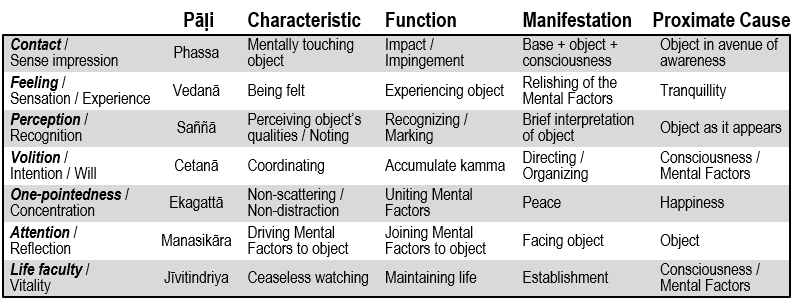
\includegraphics[width=0.8\linewidth]{./Diagrams/U-E}
\caption{Seven Universal Ethically-Variable Mental Factors}
\label{fig:U-E}
\end{figure}

Let’s start our review of Handout 3 with the seven universal ethically-variable Mental Factors starting with \textbf{Contact}.

The first ethically-variable Mental Factor is \textbf{Contact}.\footnote{Defined in Visuddhimagga XIV.134, explained in Chapter 2 of “Cetasikas” (see footnote 2).} The Suttas explain that when a \textbf{Visible-form} strikes the sensitive part of the eye, eye-consciousness arises naturally. The meeting of the three (\textbf{Visible-form}, sensitive part of the eye and eye-consciousness), is defined as \textbf{Contact}.\footnote{MN 48: \url{http://www.accesstoinsight.org/tipitaka/mn/mn.148.than.html\#phassa}} From this definition, we can see that \textbf{Contact} is not physical impact, but rather sense impression. This is why the Suttas define \textbf{Contact} according to which sense is involved: eye-\textbf{Contact}, ear-\textbf{Contact}, nose-\textbf{Contact}, tongue-\textbf{Contact}, body-\textbf{Contact} and mind-\textbf{Contact}. Dependent origination states that the six senses are a condition for the arising of \textbf{Contact} and, in turn, \textbf{Contact} is a condition for the arising of the next ethically-variable Mental Factor, \textbf{Feeling}.

We have already discussed the Mental Factor of \textbf{Feeling} in the previous talk.\footnote{Defined in Visuddhimagga XIV.125, explained in Chapter 3 of “Cetasikas” (see footnote 2).}

\textbf{Perception} is the next Mental Factor.\footnote{Defined in Visuddhimagga XIV.129, explained in Chapter 4 of “Cetasikas” (see footnote 2).} In the previous talk, I discussed perception at a high level in the stories of the snake, the coin and the elephant. Now as part of a Thought Moment, the Mental Factor Perception is working at a microscopic level.\footnote{AN 6.63: \url{http://www.accesstoinsight.org/tipitaka/an/an06/an06.063.than.html\#part-3}\\SN 27.6: \url{http://www.accesstoinsight.org/tipitaka/sn/sn27/sn27.001-010.than.html\#sn27.006}}

In the story of the man who misperceived a coil of rope as a snake, misperception happened in a fraction of a second, but this was long enough for millions of processes to occur. There were many sensing processes to capture \textbf{Visible-forms}. There were many thinking processes that integrated these \textbf{Visible-forms} to grasp the scene as a whole; many thinking processes that recognized colours in the scene, many that grasped a shape based on differentiated colours, and many that recognized a shape based on past experience. Many thinking processes associated the name “snake” with the recognized shape. Within each of these many processes, there are multiple Thought Moments, and each Thought Moment has a Mental Factor of \textbf{Perception}. So \textbf{Perception}, or in this case misperception, works at a high level, but as a Mental Factor, \textbf{Perception} also works on a microscopic level within a Thought Moment.

Within a Thought Moment, there are two roles for the Mental Factor \textbf{Perception}: first, to mark the object so it can be recognized later and second, to recognize the object that has been previously marked. These two roles allow an object to be passed between Thought Moments and processes without being forgotten, all working at a microscopic level.

Now on to \textbf{Volition}, the next Mental Factor.\footnote{Defined in Visuddhimagga XIV.135, explained in Chapter 5 of “Cetasikas” (see footnote 2).} \textbf{Volition} organizes and coordinates consciousness and all the Mental Factors to work together as a team. \textbf{Volition} plays this managerial role in all Thought Moments. In kamma-producing Thought Moments, the first row in the Thought Moments handout, \textbf{Volition} has an additional responsibility of creating new kamma. The Buddha said, “\textbf{Volition} is kamma,” so kamma comes from the mind, not from speech or action\footnote{AN 6.63: \url{http://www.accesstoinsight.org/tipitaka/an/an06/an06.063.than.html}}. Of course, all speech and actions start in the mind, and it is in the mind that kamma is created. In kamma-creating Thought Moments, \textbf{Volition} is like the manager who also rolls up his sleeves and gets things done; the extra force generates kamma. We will discuss kamma in detail in a later talk.

Moving on to \textbf{One-pointedness}.\footnote{Defined in Visuddhimagga XIV.139, explained in Chapter 7 of “Cetasikas” (see footnote 2).} The commentaries equate \textbf{One-pointedness} with concentration.\footnote{Visuddhimagga III.2 (See footnote 2).} Some translators use the term “unification of mind” or “singleness of mind” for \textbf{One-pointedness}. \textbf{One-pointedness} is like water that binds together several substances to form one concrete mass; it allows the Thought Moment to focus on one object. \textbf{One-pointedness} is ethically-variable. There can be a high degree of \textbf{One-pointedness} in unwholesome Thought Moments, such as when a hunter aims his gun. There can be a high degree of \textbf{One-pointedness} during wholesome Thought Moments, such as during meditation.\footnote{The \textit{Dhammasaṅgaṇī} mentions that all the Thought Moments that create new kamma except Thought Moment \textbf{11} (associated with \textbf{Doubt}) include self-collectedness, faculty of concentration, power of concentration, right concentration path factor, quiet and balance (all of these are synonyms for \textbf{One-pointedness}). Thought Moments \textbf{11}, \textbf{13}--\textbf{27} and \textbf{39}--\textbf{46} only include self-collectedness but not the other items; this suggests that \textbf{One-pointedness} is present, but quite weak in Thought Moments \textbf{11}, \textbf{13}--\textbf{27} and \textbf{39}--\textbf{46}.}

The next Mental Factor is \textbf{Attention}.\footnote{Defined in Visuddhimagga XIV.152, explained in Chapter 8 of “Cetasikas” (see footnote 2).} At the microscopic level, inside the Thought Moment, \textbf{Attention} acts like the rudder of a ship, directing, steering or turning consciousness and all of the Mental Factors towards the object. At a high level, \textbf{Attention}, particularly wise \textbf{Attention}, plays an important role in the practice.

The Buddha identified the two most important factors for spiritual development.\footnote{Iti 1.16: \url{http://www.accesstoinsight.org/tipitaka/kn/iti/iti.1.001-027.than.html\#iti-016}\\Iti 1.17: \url{http://www.accesstoinsight.org/tipitaka/kn/iti/iti.1.001-027.than.html\#iti-017}} The most important external factor is a good friend, a noble friend in the Dhamma. The most important internal factor is wise \textbf{Attention}. Wise \textbf{Attention} means looking at the current situation through the lens of the Dhamma. Wise \textbf{Attention} can be applied at all times, but to establish it as a habit, I have found it useful before eating to reflect on the Buddha’s advice that he gave to monks about food, “use this food not for intoxication, not for physical beauty, but simply for the survival and continuance of the body, for assisting in the practice. Avoid hunger. Avoid overeating.”

When things happen, it is often useful to apply wise \textbf{Attention} and reflect on the eight worldly conditions mentioned by the Buddha: gain and loss, fame and obscurity, praise and blame, pleasure and pain, not to be attracted to one or repelled by the other.

Scanning handout 3, you can see that wise \textbf{Attention} is a proximate cause for many of the beautiful Mental Factors, and that unwise \textbf{Attention} is a proximate cause for many of the unwholesome Mental Factors.

The final universal ethically-variable Mental Factor is \textbf{Life faculty}.\footnote{Defined in Visuddhimagga XIV.138, explained in Chapter 8 of “Cetasikas” (see footnote 2).} The function of \textbf{Life faculty} is to sustain the life of consciousness and the Mental Factors, but only for the brief instant that they exist.

Turning to Handout 4, you can see that the seven universal ethically-variable Mental Factors arise in all Thought Moments. The first column titled “Universal Ethically-variable,” which represents this group of seven Mental Factors is grey for all rows.

\begin{figure}[h]
\centering
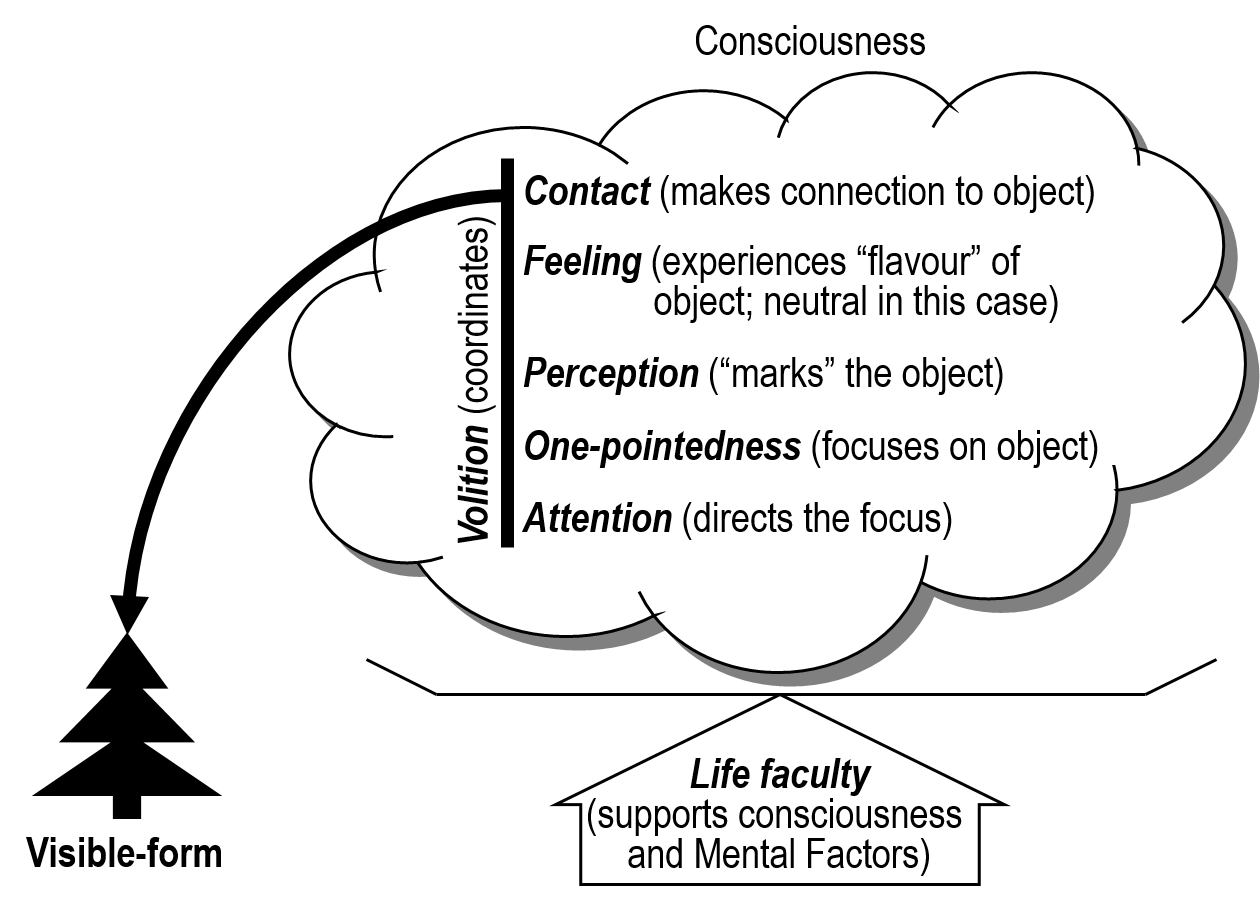
\includegraphics[width=0.7\linewidth]{./Diagrams/Eye-cons}
\caption{The 7 universal Mental Factors work as a team in the eye-consciousness Thought Moment.}
\label{fig:Eye-cons}
\end{figure}

Let’s consider how consciousness and the Mental Factors in Thought Moment \textbf{13}, eye-consciousness, work as a team. I selected this Thought Moment as an example because it has only the universal ethically-variable Mental Factors. According to the Suttas, eye-consciousness arises naturally when there is a working eye and \textbf{Visible-form}, something to be seen. Using modern terminology, the function of eye-consciousness is to capture the photograph as it appears at the retina.

Within this eye-consciousness Thought Moment, consciousness is aware of the \textbf{Visible-form}. \textbf{Contact} makes a mental connection to the \textbf{Visible-form}. \textbf{Feeling} experiences the flavour of the \textbf{Visible-form}; as we can see from the Thought Moments handout, the \textbf{Feeling} is indifferent. \textbf{Perception} marks and recognizes this \textbf{Visible-form}; multiple related photographs may be necessary to support later thinking, so \textbf{Perception} bundles past, present and future photographs into a set. This is not what we normally refer to as memory; \textbf{Perception} is much more superficial. \textbf{Volition} coordinates the activities of consciousness and the associated Mental Factors so they work as a team; the eye-consciousness Thought Moment does not create new kamma, so in this Thought Moment, \textbf{Volition} only coordinates and does not create new kamma. \textbf{One-pointedness} unifies consciousness and the Mental Factors so they are focused. \textbf{Attention} directs the focus provided by \textbf{One-pointedness} to the \textbf{Visible-form}. \textbf{Life faculty} breathes life into consciousness and into the set of Mental Factors.

Though I am presenting them in sequence, consciousness and all Mental Factors arise together and perform their respective activities at the same time. All Mental Factors interact and support each other simultaneously.

\subsubsection*{Occasionals}

\begin{figure}[h]
\centering
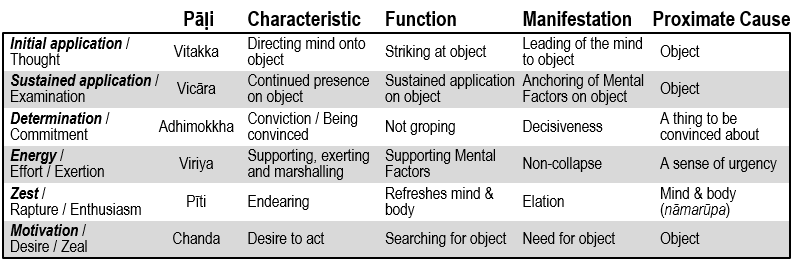
\includegraphics[width=0.8\linewidth]{./Diagrams/O-E}
\caption{Six Occasional Ethically-Variable Mental Factors}
\label{fig:O-E}
\end{figure}

We now consider the six occasional ethically-variable Mental Factors, starting with \textbf{Initial application} and \textbf{Sustained application}.\footnote{Defined in Visuddhimagga IV.88, explained in Chapter 9 of “Cetasikas” (see footnote 2).} These two Mental Factors are closely related. At a high level, \textbf{Initial application} is sometimes translated as “Thought,” but at a microscopic level, \textbf{Initial application} directs the mind onto the object. At a high level, \textbf{Sustained application} is sometimes translated as “Examination,” but at a microscopic level, \textbf{Sustained application} keeps the mind on the object. As an analogy, when I am washing a plate, one hand holds the plate while the other hand rubs the wash cloth over its surface. The hand holding the plate is \textbf{Initial application} while the hand rubbing with the wash cloth is \textbf{Sustained application}.

The next Mental Factor is \textbf{Determination}.\footnote{Defined in Visuddhimagga XIV.151, explained in Chapter 10 of “Cetasikas” (see footnote 2).} \textbf{Determination} is decisiveness. If one decides to study the Dhamma, there is wholesome \textbf{Determination}. If one complains, unwholesome \textbf{Determination} arises which is convinced that the object of \textbf{Aversion} is unacceptable.

\textbf{Energy} is the next Mental Factor.\footnote{Defined in Visuddhimagga XIV.137, explained in Chapter 10 of “Cetasikas” (see footnote 2).} The Commentary explains that when rightly initiated, \textbf{Energy} is the root of all attainments, but strong Energy can also increase the weightiness of the kamma generated by unwholesome Thought Moments. Just as a string of a musical instrument needs to be “not too tight and not too loose,” \textbf{Energy} must be exerted at the appropriate level for spiritual development.\footnote{AN 6.55: \url{http://www.accesstoinsight.org/tipitaka/an/an06/an06.055.than.html}}

Now let’s look at \textbf{Zest}.\footnote{Defined in Visuddhimagga IV.94, explained in Chapter 12 of “Cetasikas” (see footnote 2).} \textbf{Zest} takes an interest in the object and refreshes the mind and body. \textbf{Zest} generally arises in Thought Moments accompanied by pleasant \textbf{Feeling}. \textbf{Zest} is the precursor of pleasant \textbf{Feeling}; an exhausted man in a desert experiences \textbf{Zest} when seeing an oasis, he experiences pleasant \textbf{Feeling} when going into the shade and drinking the water.

The final ethically-variable Mental Factor is \textbf{Motivation}.\footnote{Defined in Visuddhimagga XIV.150, explained in Chapter 13 of “Cetasikas” (see footnote 2).} Every action begins with \textbf{Motivation}. The Commentary\footnote{See Visuddhimagga IV.63 (see footnote 2).} lists eight things that can be reflected upon to raise one’s sense of spiritual urgency: birth, ageing, sickness, death, suffering in the woeful planes, suffering from past lives, suffering in future lives, suffering in the present life rooted in the search for food.\footnote{In AN 3.38 (\url{http://www.accesstoinsight.org/tipitaka/an/an03/an03.038.than.html}) the Buddha explained his own \textbf{Motivation} for renunciation. Reflecting that he was subject to ageing, he overcame the “intoxication of youth”. Reflecting that he was subject to illness, he overcame the “intoxication of health”. Reflecting that he was subject to death, he overcame the “intoxication of life”.} A journey of 1000 miles starts with a single step, and that single step arises because of \textbf{Motivation}. This reminds me of a joke... how many Buddhas does it take to change a light bulb? None. The change must come from within, the Buddhas only show the way to change the light bulb.

Turning to Handout 4, you can see that each of the six occasional ethically-variable Mental Factors has its own column.

Looking at the Thought Moments in the Danger Zone, Thought Moments \textbf{1}--\textbf{12}, we can see that all of the occasional ethically-variable Mental Factors arise in all of the unwholesome Thought Moments with a few exceptions. Determination does not arise in Thought Moment \textbf{11}, which is associated with \textbf{Doubt}. \textbf{Zest} arises only in Thought Moments with pleasant \textbf{Feeling}. \textbf{Motivation} arises only in \textbf{Attachment}-rooted or \textbf{Aversion}-rooted Thought Moments.

Looking at the Thought Moments in the Faultless Zone, Thought Moments \textbf{31}--\textbf{38}, we can see that all occasional ethically-variable Mental Factors arise in all wholesome Thought Moments with one exception. \textbf{Zest} arises only in Thought Moments with pleasant \textbf{Feeling}.

Now let’s look at the five jhānas. The first jhāna, Thought Moment \textbf{55}, has all of the occasional ethically-variable Mental Factors.\footnote{In MN 111 (\url{http://www.accesstoinsight.org/tipitaka/mn/mn.111.than.html}), the Buddha praises Sāriputta because he is able to identify Mental Factors when examining his own mind. The Mental Factors listed in the Sutta includes all of the ethically-variable Mental Factors except \textbf{Life faculty}: \textbf{Contact} (\textit{phassa}), \textbf{Feeling} (\textit{vedanā}), \textbf{Perception} (\textit{saññā}), \textbf{Volition} (\textit{cetanā}), \textbf{One-pointedness} (\textit{ekaggatā}), \textbf{Attention} (\textit{manasikāra}), \textbf{Initial application} (\textit{vitakka}), \textbf{Sustained application} (\textit{vicāra}), \textbf{Determination} (\textit{adhimokkha}), \textbf{Energy} (\textit{viriya}), \textbf{Zest} (\textit{pīti}) and \textbf{Motivation} (\textit{chanda}).} The second jhāna, Thought Moment \textbf{56}, drops the Mental Factor of \textbf{Initial application}. The third jhāna, Thought Moment \textbf{57}, drops the Mental Factor of \textbf{Sustained application}. The fourth jhāna, Thought Moment \textbf{58}, drops the Mental Factor of \textbf{Zest}. The fourth jhāna is the only Thought Moment accompanied by pleasant \textbf{Feeling} in which \textbf{Zest} does not arise. In the fifth jhāna, Thought Moment \textbf{59}, pleasant \textbf{Feeling} is replaced with indifferent \textbf{Feeling} so there is no change in the number of Mental Factors.

\subsection*{Unwholesome Mental Factors}

\subsubsection*{Universals}

\begin{figure}[h]
\centering
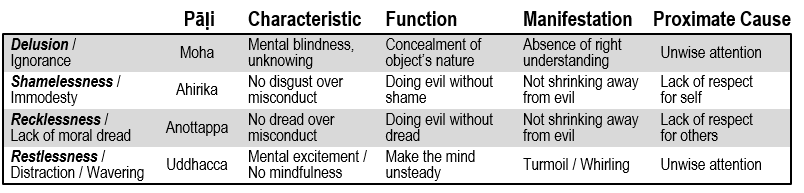
\includegraphics[width=0.8\linewidth]{./Diagrams/U-U}
\caption{Four Universal Unwholesome Mental Factors}
\label{fig:U-U}
\end{figure}

Let’s move on to the four universal unwholesome Mental Factors of \textbf{Delusion}, \textbf{Shamelessness}, \textbf{Recklessness} and \textbf{Restlessness}. These four Mental Factors are part of all unwholesome Thought Moments.

\textbf{Delusion} is considered to be the mother of all that is unwholesome.\footnote{Defined in Visuddhimagga XIV.163, explained in Chapter 15 of “Cetasikas” (see footnote 2). \textbf{Delusion} is suppressed by observing the true nature of phenomena. \textbf{Delusion} cannot be uprooted by merely thinking about realities; it can eventually be uprooted by the wisdom that knows the true nature of realities (Study → Practice → Realization). The Sotāpanna uproots \textbf{Delusion} associated with \textbf{Doubt}. The Arahat completely uproots \textbf{Delusion}.} We have already discussed the Mental Factor of \textbf{Delusion} in the previous talk.

The next Mental Factor is \textbf{Shamelessness}.\footnote{Defined in Visuddhimagga XIV.160, explained in Chapter 15 of “Cetasikas” (see footnote 2). \textbf{Shamelessness} is suppressed by considering one’s reputation. The Arahat uproots \textbf{Shamelessness}.} Just as a pig is not ashamed to roll in sewage, the mind is not disgusted with unwholesome actions, speech or thought. The Buddha said to his seven-year-old son, “When anyone feels no shame in telling a deliberate lie, there is no evil he will not do. Thus, Rahula, you should train yourself, `I will not tell a deliberate lie even in jest.’ ” \footnote{MN 61: \url{http://www.accesstoinsight.org/tipitaka/mn/mn.061.than.html\#fnt-2}} In other words, there is no room for “white lies.” To check if there is \textbf{Shamelessness} in the mind, I ask myself, “Is this the kind of Thought Moment that could arise in an Arahat?” or I ask myself, “Would I be proud if my thought were reported as a headline in tomorrow’s newspaper?”

\textbf{Recklessness} is the next Mental Factor.\footnote{Defined in Visuddhimagga XIV.160, explained in Chapter 15 of “Cetasikas” (see footnote 2). \textbf{Recklessness} is suppressed by considering the consequences of one’s action. The Arahat uproots \textbf{Recklessness}.} Just as a moth is attracted to fire and is burned, \textbf{Recklessness} is unaware of consequences, is attracted by the unwholesome and plunges into the Danger Zone. To check if there is \textbf{Recklessness} in the mind, I ask myself, “Is this Thought Moment going to be the wind under my wings to lift me up, or the weight around my neck to drag me down?” or I ask myself, “What kind of kamma is this Thought Moment creating?”

The final universal unwholesome Mental Factor is \textbf{Restlessness}.\footnote{Defined in Visuddhimagga XIV.165, explained in Chapter 15 of “Cetasikas” (see footnote 2). According to the commentary to the \textit{Satipaṭṭhāna} Sutta, \textbf{Restlessness} is suppressed through: 1) Knowledge of the Buddhist scriptures (Doctrine and Discipline); 2) Asking questions about them; 3) Familiarity with the Vinaya (the Code of Monastic Discipline, and for lay followers, with the five precepts); 4) Association with those mature in age and experience, who possess dignity, restraint and calm; 5) Noble friendship; 6) Suitable conversation. The Arahat uproots \textbf{Restlessness}.} We have already discussed the Mental Factor of \textbf{Restlessness} in the previous talk.

Handout 4 shows that the group of four universal unwholesome Mental Factors are part of Thought Moments \textbf{1}--\textbf{12} but are not part of any other Thought Moments.

\subsubsection*{Occasionals}

\begin{figure}[h]
\centering
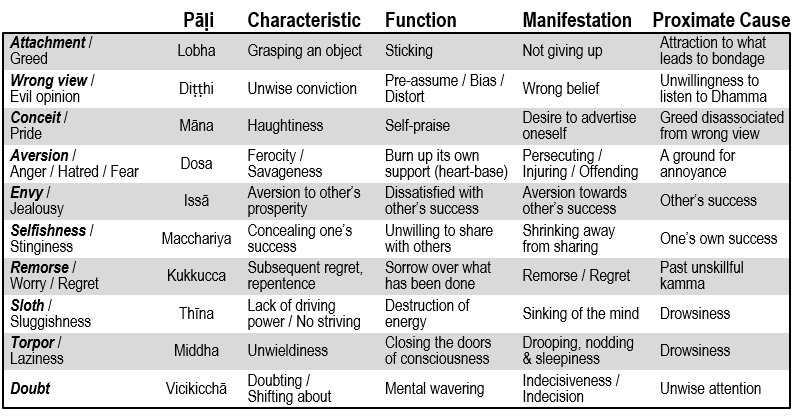
\includegraphics[width=0.8\linewidth]{./Diagrams/O-U}
\caption{Ten Occasional Unwholesome Mental Factors}
\label{fig:O-U}
\end{figure}

The first occasional unwholesome Mental Factor is \textbf{Attachment}.\footnote{Defined in Visuddhimagga XIV.162, explained in Chapter 16 of “Cetasikas” (see footnote 2). For a layperson, \textbf{Attachment} is suppressed through \textit{dāna}. According to the commentary to the \textit{Satipaṭṭhāna} Sutta, \textbf{Attachment} is suppressed through: 1) Learning how to meditate on impure objects; 2) Devoting oneself to the meditation on the impure; 3) Guarding the sense doors; 4) Moderation in eating; 5) Noble friendship; 6) Suitable conversation. The Sotāpanna uproots \textbf{Attachment} associated with \textbf{Wrong view}. The Sakadāgāmī weakens sensuous clinging. The Anāgāmī uproots sensuous clinging. The Arahat uproots clinging to existence.
} We have already discussed the Mental Factor of \textbf{Attachment} in the previous talk.

The next Mental Factor is \textbf{Wrong view}.\footnote{Defined in Visuddhimagga XIV.164, explained in Chapter 17 of “Cetasikas” (see footnote 2).} Actually, it is \textbf{Attachment} to \textbf{Wrong view}. We discussed this Mental Factor in some detail during the last talk.

\textbf{Conceit} is the next Mental Factor.\footnote{Defined in Visuddhimagga XIV.168, explained in Chapter 18 of “Cetasikas” (see footnote 2).}  \textbf{Conceit} includes all forms of comparison; “better than,” “equal to” and “inferior to.” Racism, bigotry, prejudice and competitiveness are all forms of \textbf{Conceit}.

We also previously talked about \textbf{Aversion}.\footnote{Defined in Visuddhimagga XIV.171, explained in Chapter 19 of “Cetasikas” (see footnote 2). According to the commentary to the \textit{Satipaṭṭhāna} Sutta, \textbf{Aversion} is suppressed through: 1) Learning how to meditate on loving-kindness; 2) Devoting oneself to the meditation of loving-kindness; 3) Considering that one is the owner and heir of one’s actions (kamma); 4) Frequent reflection on: “Being angry with another person, what can you do to him? Can you destroy his virtue and his other good qualities? Have you not come to your present state by your own actions, and will also go hence according to your own actions? Anger towards another is just as if someone wishing to hit another person takes hold of glowing coals, or a heated iron-rod, or of excrement. And, in the same way, if the other person is angry with you, what can he do to you? Can he destroy your virtue and your other good qualities? He too has come to his present state by his own actions and will go hence according to his own actions. Like an unaccepted gift or like a handful of dirt thrown against the wind, his anger will fall back on his own head.”; 5) Noble friendship; 6) Suitable conversation. The Sakadāgāmī weakens \textbf{Aversion}. The Anāgāmī uproots \textbf{Aversion}.}

Moving on to \textbf{Envy}; \textbf{Envy} is outward looking, it focuses on others.\footnote{Defined in Visuddhimagga XIV.172, explained in Chapter 20 of “Cetasikas” (see footnote 2).} For example, \textbf{Envy} arises when we are dissatisfied because we feel that somebody’s life is better than ours. The mind can be trained to reduce the negative mental habit of \textbf{Envy} by developing the positive habit of \textbf{Sympathetic joy}.

The next Mental Factor is \textbf{Selfishness}; \textbf{Selfishness} is inward looking, it focuses on ourselves.\footnote{Defined in Visuddhimagga XIV.173, explained in Chapter 20 of “Cetasikas” (see footnote 2).} When I am overcome by \textbf{Selfishness}, I consider that there are no things I can possess; phenomena rise and fall away cannot belong to me.

There was a fun film almost 30 years ago called “Crocodile Dundee” \footnote{\url{http://en.wikipedia.org/wiki/Crocodile_Dundee}} and I still remember one of the quotes from that film, “Aborigines don’t own the land. They belong to it. It’s like their mother. See those rocks? Been standing there for 600 million years. Still be there when you and I are gone. So arguing who owns them is like two fleas arguing over who owns the dog they live on.”

Why are we stingy about what does not belong to us? We cannot take our possessions with us when we die. Life is so short; we waste many opportunities for wholesome actions because of our stinginess. We can reduce accumulation of \textbf{Selfishness} by practising generosity.

\textbf{Remorse} is the next Mental Factor.\footnote{Defined in Visuddhimagga XIV.174, explained in Chapter 20 of “Cetasikas” (see footnote 2).} The Commentary refers to \textbf{Remorse} as a state of bondage. When there is \textbf{Remorse}, there is also \textbf{Aversion} towards the past object.\footnote{Iti 30: \url{http://www.accesstoinsight.org/tipitaka/kn/iti/iti.2.028-049.than.html\#iti-030}} The proper way of dealing with \textbf{Remorse} is not to dwell on it but rather to acknowledge, forgive yourself and learn. Acknowledge, forgive and learn are the underlying principles of the Vinaya. Repentance is considered a virtue, but \textbf{Remorse} is unwholesome. \textbf{Remorse} that regrets unwholesome deeds and the non-arising of wholesome deeds is different from thinking about the disadvantages of unwholesome deeds and the value of wholesome deeds. The Suttas explain that virtuous behaviour leads to freedom from \textbf{Remorse} and freedom from \textbf{Remorse} can lead to becoming an Arahat.\footnote{AN 11.1: \url{http://www.accesstoinsight.org/tipitaka/an/an11/an11.001.than.html}}

Now let’s look at \textbf{Sloth} and \textbf{Torpor}.\footnote{Defined in Visuddhimagga XIV.167, explained in Chapter 21 of “Cetasikas” (see footnote 2).} These two Mental Factors always arise together and make the mind unwieldy and lazy. The Commentary refers to \textbf{Sloth} and \textbf{Torpor} as paralysis due to lack of urgency and lack of energy. \textbf{Sloth} is called a sickness of consciousness while \textbf{Torpor} is called a sickness of the other Mental Factors.

All Thought Moments in the Danger Zone and in the Faultless Zone have the Mental Factor of \textbf{Energy}. In some Thought Moments, \textbf{Energy} is more intense and in other Thought Moments, \textbf{Energy} is less intense. The Thought Moments in which \textbf{Energy} is less intense rely on external factors and are prompted. When Thought Moments in the Danger Zone have less intense \textbf{Energy}, this is a condition for \textbf{Sloth} and \textbf{Torpor} to arise.

The final unwholesome Mental Factor is \textbf{Doubt}.\footnote{Defined in Visuddhimagga XIV.177, explained in Chapter 21 of “Cetasikas” (see footnote 2).} \textbf{Doubt} was discussed in the previous talk.

\begin{figure}[h]
\centering
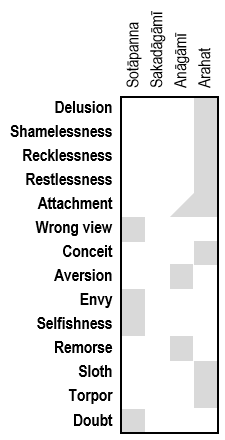
\includegraphics[width=0.3\linewidth]{./Diagrams/Freedom}
\caption{The stages at which the saint becomes free from unwholesome Mental Factors. The Anāgāmī is free from \textbf{Attachment} to sense objects and an Arahat is free from all \textbf{Attachment}, including craving for fine-material existence and craving for immaterial existence.}
\label{fig:Freedom}
\end{figure}

Imagine that the unwholesome Mental Factors were people and they were having a discussion after a retreat. \textbf{Delusion} says, “Things would be better if only...;” \textbf{Shamelessness} says, “I’m not embarrassed if I disturb other yogis;” \textbf{Recklessness} says, “The teacher didn’t catch me when I stayed in bed;” \textbf{Restlessness} says, “When is the next retreat?” \textbf{Attachment} says, “I enjoyed the food at this centre;” \textbf{Wrong view} says, “There is only one way to practice;” \textbf{Conceit} says, “I am the best practitioner of the group;” \textbf{Aversion} says, “I did not like the attitude of the teacher;” \textbf{Envy} says, “I wish I could practice like the other yogi;” \textbf{Selfishness} keeps quiet because he wants to keep what he has learned to himself, does not want to share; \textbf{Remorse} says, “I should have been more diligent;” \textbf{Sloth} says, “I couldn’t be bothered to practice;” \textbf{Torpor} says, “I was too tired to practice” and \textbf{Doubt} says, “Not sure if practice has any benefit.” It is ironic that even a retreat can be fuel for unwholesome Mental Factors to arise.

The Suttas often list five factors that are hindrances\footnote{\url{http://en.wikipedia.org/wiki/Five_hindrances}} to spiritual progress, and provide an analogy of how conditions make it difficult to see things as they truly are.\footnote{SN 46.55: \url{http://www.accesstoinsight.org/tipitaka/sn/sn46/sn46.055.wlsh.html}} The first hindrance is sense-desire; this is \textbf{Attachment} to the current situation. Sense-desire is like mixing many colours in a bowl of water, making it difficult to see one’s reflection. The second hindrance is ill will; this is \textbf{Aversion}, not accepting the current situation. Ill will is like boiling a bowl of water, making it difficult to see one’s reflection. The third hindrance is \textbf{Sloth} and \textbf{Torpor}; sluggishness and laziness. \textbf{Sloth} and \textbf{Torpor} are like the bowl of water being covered in moss, making it difficult to see one’s reflection. The fourth hindrance is \textbf{Restlessness} and \textbf{Remorse}. \textbf{Restlessness} and \textbf{Remorse} are like the wind agitating the surface of the bowl of water, making it difficult to see one’s reflection. The fifth hindrance is \textbf{Doubt}. \textbf{Doubt} is like muddy water in the bowl, making it difficult to see one’s reflection.

The Commentary gives a useful summary of practices to overcome each of these hindrances.\footnote{This list was taken from page 200 of \url{http://www.buddhismuskunde.uni-hamburg.de/pdf/5-personen/analayo/direct-path.pdf}} The one practice that is common to overcome all five hindrances is “good friends and suitable conversation.” In one Sutta, Ānanda said to the Buddha that having good friends was half of the holy life.\footnote{SN 45.2: \url{http://www.accesstoinsight.org/tipitaka/sn/sn45/sn45.002.than.html}; the footnote to this Sutta explains that “good friends” means not only associating with good people, but also learning from them and emulating their good qualities.} The Buddha replied that having good friends was the whole of the holy life, because the Buddha was a good friend, others can gain liberation.

The Commentary suggests that to overcome sensual desire, one should learn and practice the 32 parts of the body mediation (as explained in paragraph 14 of the \textit{Satipaṭṭhāna} Sutta), should guard the senses and practice moderation in eating.\footnote{See also Iti 29: \url{http://www.accesstoinsight.org/tipitaka/kn/iti/iti.2.028-049.than.html}}

The Commentary suggests that to overcome ill will, one should learn and practice mettā meditation, reflect on the kammic consequences of one’s actions, and repeatedly look at things with wise \textbf{Attention} through the lens of the Dhamma.

The Commentary suggests that to overcome \textbf{Sloth} and \textbf{Torpor}, one should lessen food intake, occasionally change your meditation posture or stay outdoors.

The Commentary suggests that to overcome \textbf{Restlessness} and \textbf{Remorse}, one should study the Suttas and Vinaya, visit experienced elders and ask them questions about the Dhamma.

The Commentary suggests that to overcome \textbf{Doubt}, one should study the Suttas and Vinaya, ask questions about the Dhamma and have a strong commitment.

Before leaving the unwholesome Mental Factors, let’s look at some of the Thought Moments in which they arise. Please refer to Handout 4 and reference Handout 2.

\begin{figure}[h]
\centering
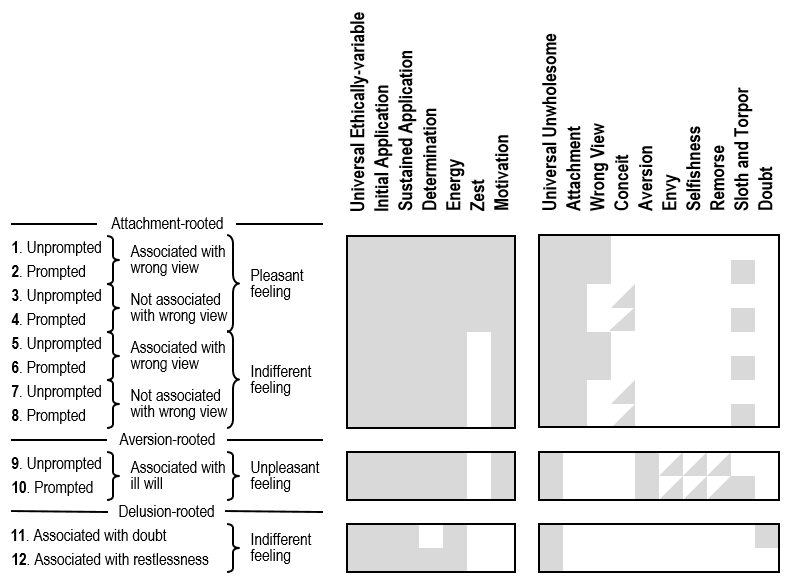
\includegraphics[width=1\linewidth]{./Diagrams/Unwholesome}
\caption{Combination of a portion of Handout 2 and a portion of Handout 4 to focus on the unwholesome Mental Factors.}
\label{fig:Unwholesome}
\end{figure}

As mentioned earlier, the four Universal Unwholesome Mental Factors, starting with \textbf{Delusion} and ending with \textbf{Restlessness}, arise in all unwholesome Thought Moments. The first column is grey for all unwholesome Thought Moments, \textbf{1}--\textbf{12}, but blank for all other Thought Moments.

\textbf{Attachment} arises in the first eight Thought Moments, but in none of the others. \textbf{Wrong view} arises in Thought Moments \textbf{1}, \textbf{2}, \textbf{5} and \textbf{6}; this can also be seen on Handout 2. \textbf{Wrong view} and \textbf{Conceit} cannot arise in the same Thought Moment because their way of taking the object is different. \textbf{Wrong view} is convinced that an object has qualities of permanence, beauty or Self, when in fact, the object has the opposite qualities of impermanence, not-to-be-clung-to and non-self. \textbf{Conceit} is an activity of comparison of beings, this being is better or worse than, or equal to another being. So, depending on the object, Thought Moments \textbf{3}, \textbf{4}, \textbf{7} and \textbf{8} can arise with or without \textbf{Conceit}. \textbf{Envy}, \textbf{Selfishness} and \textbf{Remorse} always arise together with \textbf{Aversion} because none of them accept the object as it is. \textbf{Envy}, \textbf{Selfishness} and \textbf{Remorse} each take different types of objects, so they cannot arise together. \textbf{Sloth} and \textbf{Torpor} arise in prompted Thought Moments, Thought Moments \textbf{2}, \textbf{4}, \textbf{6}, \textbf{8} and \textbf{10}. \textbf{Doubt} only arises in one Thought Moment, Thought Moment \textbf{11}.

\pagebreak

\begin{figure}[h]
\centering
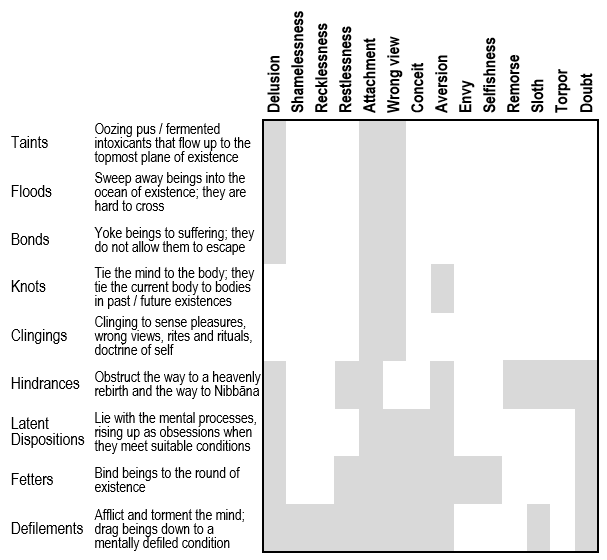
\includegraphics[width=0.75\linewidth]{./Diagrams/Groups1}
\caption{Correlation between groupings found in the Suttas and the Unwholesome Mental Factors.}
\label{fig:Groups1}
\end{figure}

\subsection*{Beautiful Mental Factors}

\subsubsection*{Universals}

\begin{figure}[h]
\centering
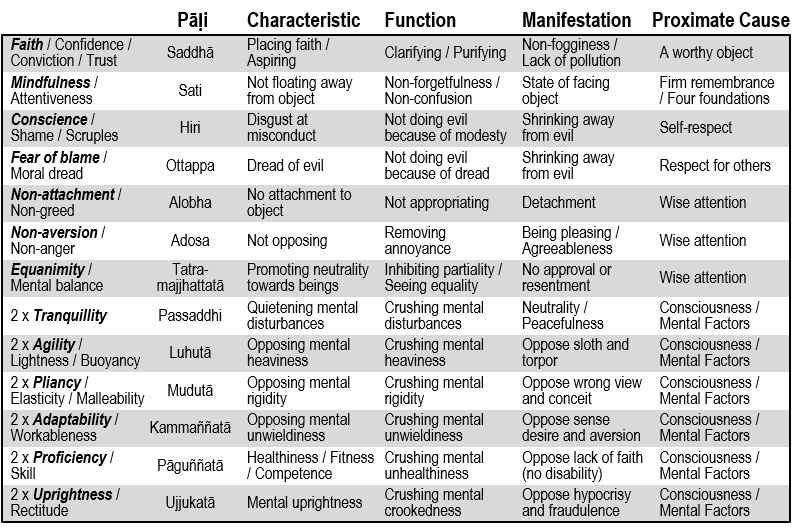
\includegraphics[width=0.8\linewidth]{./Diagrams/U-W}
\caption{Nineteen Universal Beautiful Mental Factors}
\label{fig:U-W}
\end{figure}

The third group, indicated by the number 3 on Handout 3, are the beautiful Mental Factors. This group includes \textbf{Faith} through \textbf{Abstinence from wrong livelihood}. The first subgroup is the universals and the second subgroup is the occasionals.

\begin{figure}[h]
\centering
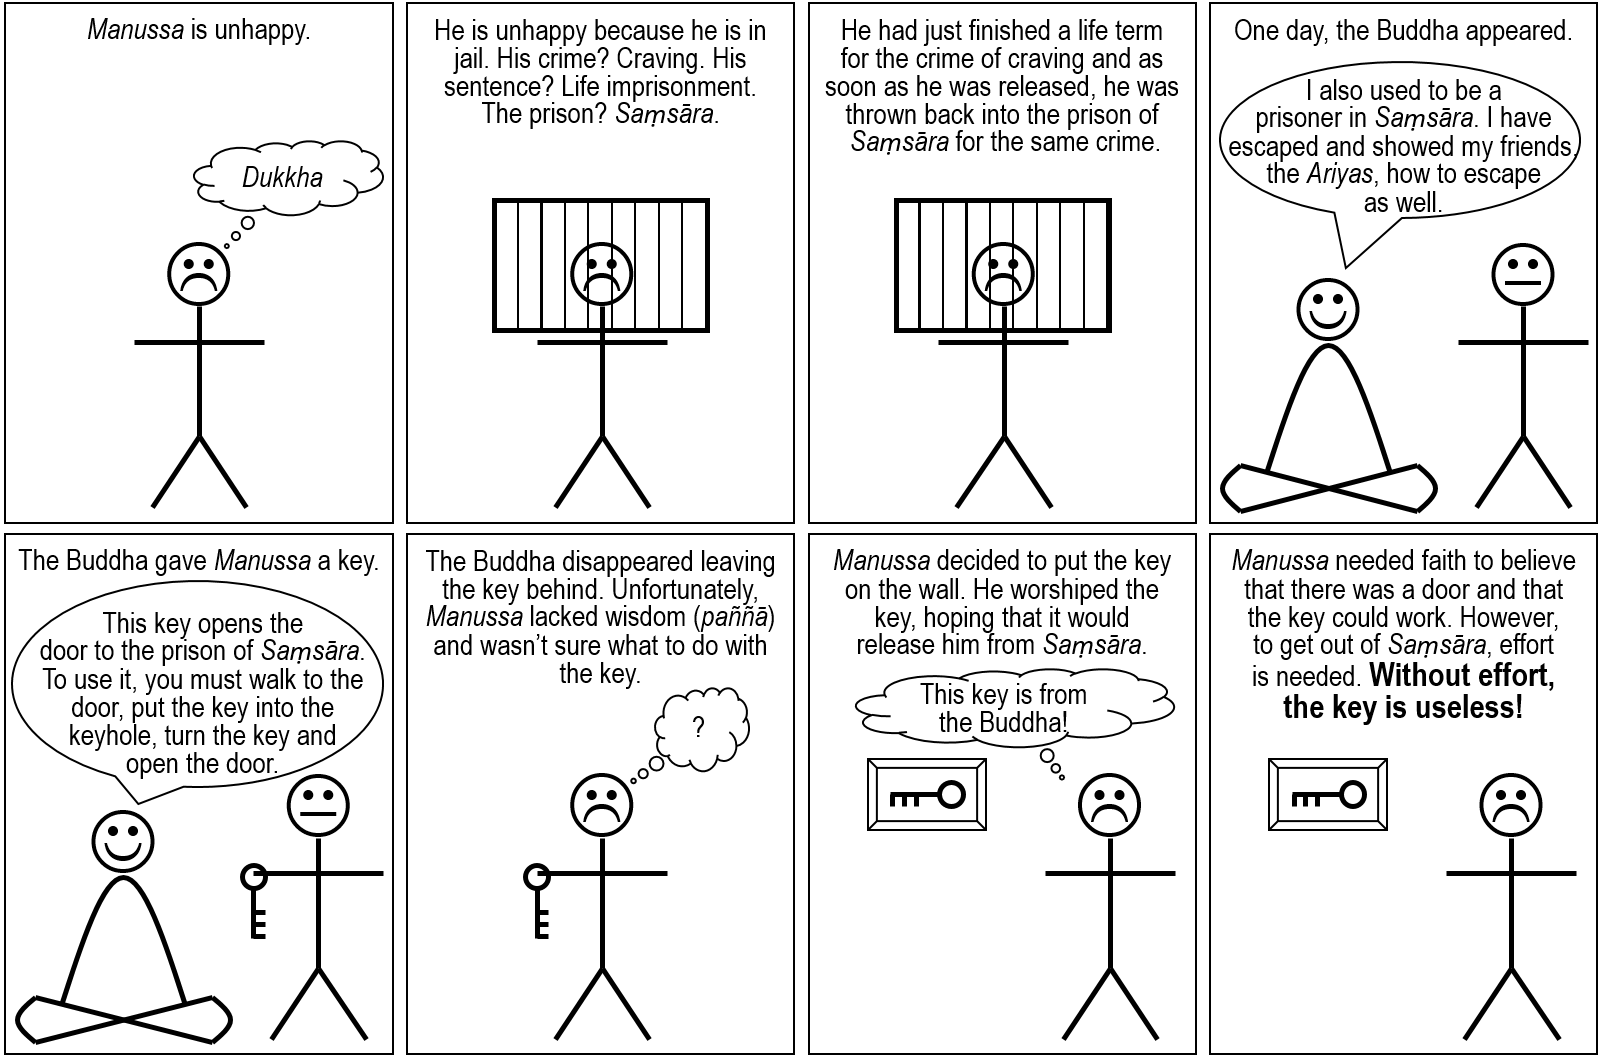
\includegraphics[width=1.0\linewidth]{./Diagrams/Key}
\caption{Manussa” is the Pāḷi word for human. “Manussa” is derived from the words for “abundance” and “mind.”}
\label{fig:Key}
\end{figure}

The first beautiful Mental Factor is \textbf{Faith}.\footnote{Defined in Visuddhimagga XIV.140, explained in Chapter 26 of “Cetasikas” (see footnote 2).} The Commentary regards \textbf{Faith} as the leader of all beautiful Mental Factors.\footnote{The five benefits of \textbf{Faith}; AN 5.38: \url{http://www.accesstoinsight.org/tipitaka/an/an05/an05.038.than.html}} When you have confidence in the value of \textit{dāna} (generosity), \textit{sīla} (discipline), or \textit{bhāvanā} (mental cultivation), you will apply yourself to it. When Buddhists take refuge in the Triple Gem, their \textbf{Faith} should be reasoned and rooted in \textbf{Understanding}. A Buddhist’s \textbf{Faith} is not in conflict with the spirit of enquiry. The Suttas discourage blind \textbf{Faith} and encourage reasoned confidence. People who have negative associations to the word “\textbf{Faith}” should substitute it with “confidence” when reading translations of Buddhist Suttas.

Shortly before his \textit{parinibbāna}, the Buddha said that there were four places that a Buddhist should visit with \textbf{Faith} to increase their sense of spiritual urgency: the place of the Buddha’s birth, enlightenment, first sermon and \textit{parinibbāna}.\footnote{DN 16: \url{http://www.accesstoinsight.org/tipitaka/dn/dn.16.5-6.than.html\#pilgrim}} I have visited these pilgrimage sites and they inspired deep reverence in me.\footnote{The leader of my tour group has published a book about Buddhist pilgrimage: \url{http://www.urbandharma.org/udharma14/pilgrim.html}}

The main benefit that I get from studying the Abhidhamma is a better understanding of the Suttas. For me, the Abhidhamma clarifies the meaning of the Suttas and this clarity instils strong confidence and \textbf{Faith} in me. This strong confidence and \textbf{Faith} motivates me to practice.

\begin{figure}[h]
\centering
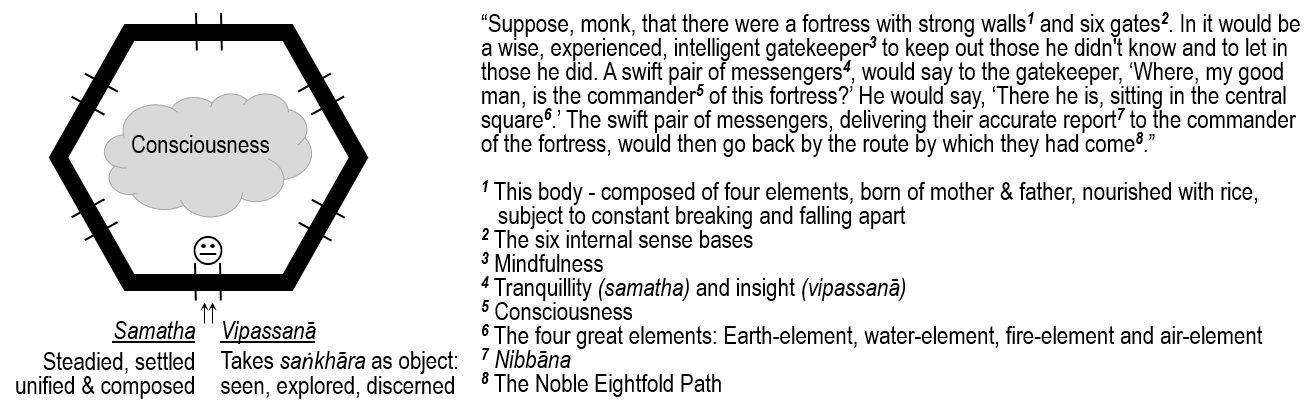
\includegraphics[width=1.0\linewidth]{./Diagrams/Fortress}
\caption{In this Sutta (SN 35.204: \url{http://www.accesstoinsight.org/tipitaka/sn/sn35/sn35.204.than.html\#fort}), the Buddha describes \textbf{Mindfulness} as a “wise, experienced, intelligent gatekeeper who keeps out those he doesn’t know and lets in those he does.”}
\label{fig:Fortress}
\end{figure}

The next Mental Factor is \textbf{Mindfulness}.\footnote{Defined in Visuddhimagga XIV.141, explained in Chapter 27 of “Cetasikas” (see footnote 2).} A modern Buddhist teacher\footnote{\url{http://en.wikipedia.org/wiki/Henepola_Gunaratana}} describes \textbf{Mindfulness}\footnote{\url{http://www.urbandharma.org/udharma4/mpe13.html}} in many different ways: Mirror-thought accurately reflects what is presently happening\footnote{Remember the cat photos illustrating \textbf{Delusion} and \textbf{Attachment} to \textbf{Wrong view}?}; there are no biases. Impartial watchfulness doesn’t take sides; no clinging to pleasant or fleeing from unpleasant. Non-conceptual awareness pays bare attention; it registers experiences, but does not compare. Present-time awareness stays forever in the present moment. Non-egoistic alertness has no reference to Self. Goalless awareness does not try to accomplish anything. Awareness of change watches the flow of the show. Non-judgemental observation: observes things in a natural state; no criticism or judgement. This is \textbf{\textit{A}}ccept in the \textbf{\textit{RADICAL}} acronym.

Mindfulness is more than just being in the present moment. As an analogy, when driving on an open highway, the mind may be in the present moment (not thinking about the past or the future) but there is no mindfulness because there is superficiality, the mind is not face to face with the object. On the other hand, mindfulness is like when you are trying to park your car in a tight spot, the mind does not float away from the object and pays close attention. Being in the present moment without mindfulness is superficial, like watching something on TV, whereas being in the present moment with mindfulness is like experiencing something in real life; experiencing it with the heart.

Consciousness is the simple awareness that is always happening. \textbf{Mindfulness} is the breakthrough observing power that comes face to face with the object. For example, when we are watching a movie in a theatre, there is consciousness or awareness of what is happening in the movie. \textbf{Mindfulness} is the realization or remembering of “I am watching a movie in a theatre.” 

Our six senses usually lead us around as if we were on a leash. \textbf{Mindfulness} wakes us up to what is really happening. \textbf{Understanding} uses \textbf{Mindfulness} as a platform and builds on \textbf{Mindfulness} through investigation. \textbf{Understanding} learns through investigation. \textbf{Understanding} can ask, “Is this wholesome or unwholesome, necessary or unnecessary?” \textbf{Understanding} can investigate what we are being mindful of, and sees that it is all just nature unfolding.

\textbf{Conscience} and \textbf{Fear of blame}\footnote{Defined in Visuddhimagga XIV.142, explained in Chapter 28 of “Cetasikas” (see footnote 2).} are the next Mental Factors. Their opposites, \textbf{Shamelessness} and \textbf{Recklessness}, were mentioned earlier as universal unwholesome Mental Factors. The Buddha referred to \textbf{Conscience} and \textbf{Fear of blame} as the bright guardians of the world because they protect society from degrading to a level of animals.\footnote{AN 2.9: \url{http://www.accesstoinsight.org/tipitaka/an/an02/an02.009.than.html}} In other words, it is not laws that protect society, it is each individual’s internal moral compass and sense of responsibility.

\begin{figure}[h]
\centering

\includegraphics[width=0.17\linewidth]{./Diagrams/AngelDevil}
\caption{\textbf{Conscience} is the angel on your shoulder and \textbf{Shamelessness} is the devil.}
\label{fig:AngelDevil}
\end{figure}

In cartoons, \textbf{Conscience} is often represented as a small angel sitting on one shoulder whispering into one ear, while bad habits are shown as a small devil sitting on the other shoulder whispering into the other ear. Constantly feeding the bad habits while ignoring \textbf{Conscience} leads to an undernourished \textbf{Conscience}. The effects of an undernourished \textbf{Conscience} are \textbf{Remorse}, reduced self-image and sometimes depression (all of these are types of \textbf{Aversion}). Reminds me of a joke... a clear conscience is usually the sign of a bad memory.

Now let’s look at \textbf{Non-attachment}.\footnote{Defined in Visuddhimagga XIV.143, explained in Chapter 29 of “Cetasikas” (see footnote 2).} \textbf{Non-attachment} is not merely the absence of \textbf{Attachment}, it counteracts \textbf{Attachment} and is the foundation of the acts of generosity, detachment and renunciation. Planning the act of giving, performing the act of giving and recalling the act of giving are all wholesome Thought Moments with \textbf{Non-attachment} toward the object that is being given. The giving of the Dhamma is superior to giving material things.\footnote{Iti 3.98: \url{http://www.accesstoinsight.org/tipitaka/kn/iti/iti.3.050-099.than.html}; also Dhammapada 354, “The gift of Dhamma excels all other gifts” (\textit{sabba dānam dhamma dānam jināti}).} Some believe that renunciation requires one to become a monk or a nun, but this is not true. Renunciation arises when you withdraw from sense pleasures, motivated by a sense of spiritual urgency. For example, at this very moment you could be gratifying your senses, indulging in sense pleasures, but you chose to study Abhidhamma. This is a form of renunciation.

In Thought Moments \textbf{33}, \textbf{34}, \textbf{37} and \textbf{38} (Thought Moments without \textbf{Understanding}) there is \textbf{Non-attachment} to the current object; for example, when offering dāna, there is \textbf{Non-attachment} to what is being given. In Thought Moments with \textbf{Understanding}, Thought Moments \textbf{31}, \textbf{32}, \textbf{35} and \textbf{36}, there is \textbf{Non-attachment} to the current object, together with an appreciation of the value of wholesome Thought Moments or a realization of non-self.

The next Mental Factor, \textbf{Non-aversion}, is the foundation for patience and loving-kindness.\footnote{Defined in Visuddhimagga XIV.143, explained in Chapter 30 of “Cetasikas” (see footnote 2).} \textbf{Non-aversion} counteracts \textbf{Aversion}. Again, this is not merely the absence of \textbf{Aversion}, it is the active opposite of \textbf{Aversion}. For example, when I am enjoying my coffee, there is \textbf{Attachment} and there is an absence of \textbf{Aversion}, but there is no patience or loving-kindness.

Patience means acceptance; it allows us to endure and tolerate both the undesirable and the desirable. We tolerate the desirable by not clinging to it.

It is valuable to instill a habit of loving-kindness, Mettā. This can be done by silently repeating a phrase such as “May all beings be well and happy.” Sometimes, this is combined with \textbf{Compassion}, “May all beings be free from suffering, may they be well and happy.” When cultivating loving-kindness, we need to be careful to ask ourselves, “Do we want to be kind only to those we like, or can we be kind to whomever we meet because we are truly concerned for their welfare?”

I once attended a Dhamma talk on Mettā given by a monk. During the Q and A session a lady asked, “One of my co-workers is nasty. I have been radiating Mettā to her for a month and she still hasn’t changed. What to do now?” The monk smiled and said, “Mettā is supposed to change you, not change the other person!”

The next Mental Factor is \textbf{Equanimity}.\footnote{Defined in Visuddhimagga XIV.153, explained in Chapter 31 of “Cetasikas” (see footnote 2).} \textbf{Equanimity} is even-mindedness, and stability that does not give a foothold to Mental Factors such as \textbf{Attachment} or \textbf{Aversion}. \textbf{Equanimity} can arise when reflecting that all things arise based on conditions, and that beings inherit their kamma. It is valuable to cultivate a habit of \textbf{Equanimity} by silently repeating a phrase such as, “May we all accept things as they are.”

We will treat the final 12 universal beautiful Mental Factors as a set. Included in this set are six pairs of Mental Factors; one of them applies to consciousness and the other applies to the remaining Mental Factors. For example, the first pair is “\textbf{Tranquillity} of consciousness” and “\textbf{Tranquillity} of Mental Factors.”

Imagine two people who have just finished listening to a Dhamma talk by Ajahn Brahm. Just to provide some context, Ajahn Brahm talks mix the Dhamma with humorous stories (a spoonful of sugar helps the medicine go down?).

The Thought Moment of person A is in the Faultless Zone while the Thought Moment of person B is in the Danger Zone. Both people experienced pleasant \textbf{Feeling}, but person A listened with joy while person B enjoyed listening. Consider the differences in experience between “listening with joy” and “enjoying listening.”

Person A experiences \textbf{Tranquillity}.\footnote{Defined in Visuddhimagga XIV.144, explained in Chapter 32 of “Cetasikas” (see footnote 2).} He is filled with calmness and warmth from being in the presence of something beautiful. He listens patiently to the Dhamma so that he will have more \textbf{Understanding}. Person B does not have \textbf{Tranquillity}. He is restless as his mind jumps between the amusing stories in the talk.

Person A experiences \textbf{Agility}.\footnote{Defined in Visuddhimagga XIV.145, explained in Chapter 32 of “Cetasikas” (see footnote 2).} He is inspired to take positive action. His mind is light and nimble, ready to quickly seize an opportunity for wholesome actions. Person B does not have \textbf{Agility}. This creates conditions for sluggishness and laziness, \textbf{Sloth} and \textbf{Torpor}, because the talk is finished and “the show is over.”

Person A experiences \textbf{Pliancy}.\footnote{Defined in Visuddhimagga XIV.146, explained in Chapter 32 of “Cetasikas” (see footnote 2).} He focuses on the application of the Dhamma as his mind naturally spreads the Dhamma learned to various aspects of his life. Person B does not have \textbf{Pliancy}. He focuses on his own enjoyment of the experience. His mind is rigid and his focus is on himself and his own viewpoints, not on the Dhamma.

Person A experiences \textbf{Adaptability}.\footnote{Defined in Visuddhimagga XIV.147, explained in Chapter 32 of “Cetasikas” (see footnote 2).} His mind is workable and flexible with just the right amount of \textbf{Pliancy}. Too much \textbf{Pliancy} makes the mind easily influenced so the Dhamma is overwritten by the next thought. Too little \textbf{Pliancy} makes the mind stubborn so that the Dhamma is ignored. Person B does not have \textbf{Adaptability}. Though he enjoyed the talk, he judges that there were both fun parts and boring parts. He likes the fun parts and dislikes the boring parts thereby making his mind less workable.

Person A experiences \textbf{Proficiency}.\footnote{Defined in Visuddhimagga XIV.148, explained in Chapter 32 of “Cetasikas” (see footnote 2).} His mind is healthy, fit and competent. It is ready to faultlessly and spontaneously apply the Dhamma from the talk into his life. Person B does not have \textbf{Proficiency}. His mind is sickly, lacking confidence to push himself to integrate the Dhamma from the talk into his own life.

Person A experiences \textbf{Uprightness}.\footnote{Defined in Visuddhimagga XIV.149, explained in Chapter 32 of “Cetasikas” (see footnote 2).} His mind is sincere. He wants to use the Dhamma from the talk to improve his spiritual development. Person B does not have \textbf{Uprightness}. He has a crafty mind, thinking about how to repeat the content of the talk to make himself look good.

To summarize these 12 Mental Factors for Person A, he listens with joy and his mind is calm, inspired, elastic, flexible, healthy and sincere. Person B enjoys listening but his mind is agitated, sluggish, rigid, judgemental, sickly and crafty. Our own mind changes very rapidly; at one moment, our mind can be wholesome like that of Person A and the next instant, our mind can be unwholesome like that of Person B.

\subsubsection*{Occasionals}

\begin{figure}[h]
\centering
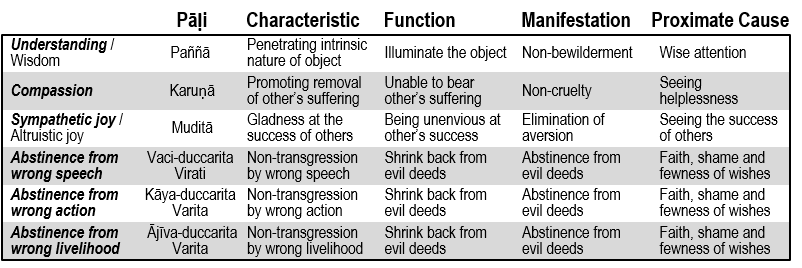
\includegraphics[width=0.8\linewidth]{./Diagrams/O-W}
\caption{Six Occasional Beautiful Mental Factors}
\label{fig:O-W}
\end{figure}

All of the beautiful Mental Factors discussed so far arise in every wholesome Thought Moment. The first occasional beautiful Mental Factor is \textbf{Understanding} or wisdom.\footnote{Defined in Visuddhimagga XIV.143, explained in Chapter 35 of “Cetasikas” (see footnote 2).}. We discussed \textbf{Understanding} in some detail in the previous talk so we will not review it here.

The next two Mental Factors, \textbf{Compassion} and \textbf{Sympathetic joy}\footnote{Defined in Visuddhimagga XIV.154, explained in Chapter 34 of “Cetasikas” (see footnote 2).} can arise when there is a suitable object.

\textbf{Compassion} arises when the mind cannot bear others’ suffering and wants to remove that suffering. It is valuable to instill a habit of \textbf{Compassion} by silently repeating a phrase such as “May all beings be free from suffering.” This may sound like loving-kindness, but the motives of loving-kindness and \textbf{Compassion} are different.

When we visit a sick person, we may offer them flowers and wish them well; these are moments of loving-kindness. When we notice their suffering, moments of \textbf{Compassion} may arise. Pity and \textbf{Aversion} sometimes displace \textbf{Compassion} without our noticing. When visiting a sick person we may have moments of \textbf{Compassion} where we wish that the person’s suffering be reduced. The next moment, we may be thinking of the person’s sickness with \textbf{Aversion} or fear. The following moment, we may be thinking with \textbf{Aversion} about the injustice of the situation. After that, we may have pity toward the person. True \textbf{Compassion} does not involve \textbf{Aversion} or pity.

When I am being scolded, I try not to allow \textbf{Aversion} to cloud my mind. I first consider how I can improve myself and also feel \textbf{Compassion} for the person doing the scolding; they are experiencing a painful \textbf{Feeling}.

I share the Abhidhamma because I believe that, if properly understood, the Abhidhamma can be useful to support one’s spiritual development. So it is out of \textbf{Compassion} for you, the listener, that I share what I hope will be helpful to you.

The Mahāyāna tradition places a lot of emphasis on \textbf{Compassion}. Here is a story from that tradition. Two monks were washing their bowls in the river when they noticed a scorpion that was drowning. One monk immediately scooped it up and set it upon the bank; in the process he was stung. He went back to washing his bowl and again the scorpion fell in, the monk saved the scorpion and was again stung. The second monk asked him, “Friend, why do you continue to save the scorpion when you know its nature is to sting?” “Because,” the first monk replied, “to save is my nature.” I have heard variations on this story, but my favourite is when the second monk takes a leaf from the ground and uses this leaf to scoop the scorpion out of the water. He showed the first monk how to save the scorpion without being stung.

\textbf{Sympathetic joy} arises when others have good fortune. When this happens, we can silently and sincerely repeat a phrase such as “may your good fortune continue.” This must be done without judgement, without comparing and especially without \textbf{Attachment}.

The final beautiful Mental Factors are the three abstinences,\footnote{Defined in Visuddhimagga XIV.155, explained in Chapter 33 of “Cetasikas” (see footnote 2).}. \textbf{Abstinence from wrong speech} means avoiding lying, slander, harsh speech and idle chatter. \textbf{Abstinence from wrong action} means avoiding killing, stealing and sexual misconduct. \textbf{Abstinence from wrong livelihood} means avoiding jobs dealing in weapons, living beings, butchery, poisons and intoxicants. 

In mundane Thought Moments, abstinences arise one at a time when the opportunity presents itself and we can abstain from only one thing at a time. There are different degrees of abstinence. Abstaining in spite of opportunity is momentary. Abstaining because of observance of precepts is temporary. Abstaining by way of eradication is permanent for saints. We may refrain from wrong speech, action or livelihood because of \textbf{Delusion} or with \textbf{Aversion}, but this is not a wholesome Thought Moment. When we abstain from wrong speech, action or livelihood with kindness and patience, this is a wholesome Thought Moment.

As the spiritual path progresses, five Mental Factors, referred to as spiritual faculties, tend to dominate the mind. They are \textbf{Faith}, \textbf{Energy}, \textbf{Mindfulness}, Concentration\footnote{Concentration is the Mental Factor of \textbf{One-pointedness}.} and \textbf{Understanding}. The Commentary stresses the importance of balancing the spiritual faculties as part of meditation. \textbf{Faith} and \textbf{Understanding} must be balanced, \textbf{Energy} and concentration must be balanced. I feel that we can apply a similar principle on a broader scale when considering our practice. \textbf{Faith}-based practice may involve chanting and attending ceremonies. \textbf{Energy}-based practice may involve volunteering and charity works. \textbf{Mindfulness}-based practice may involve \textit{vipassanā} meditation. Concentration-based practice may involve \textit{samatha} meditation. \textbf{Understanding}-based practice may involve studying and teaching the Dhamma. Just as all five fingers of the hand need to be strong and coordinated, so too the five types of practice can best support each other when each of them is equally developed. For example, you may look at yourself and say, “My practice puts a lot of emphasis on \textbf{Understanding}, but not so much on \textbf{Energy}. Perhaps I should look at ways of increasing my \textbf{Energy}-based practice by doing volunteer work.”

Before leaving the beautiful Mental Factors, let’s look at some of the Thought Moments in which they arise. Please refer to Handout 4 and reference Handout 2.

\begin{figure}[h]
\centering
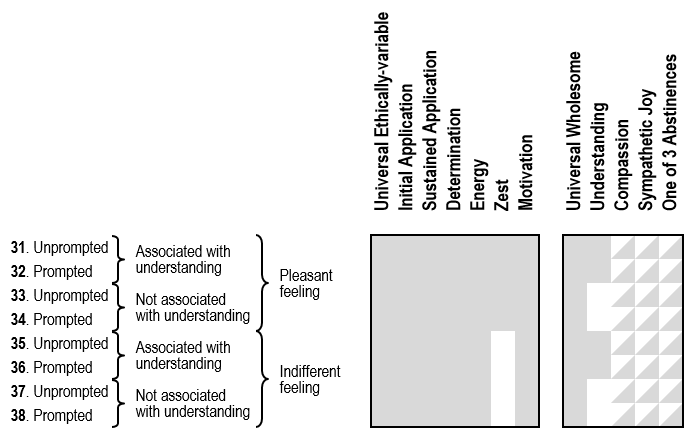
\includegraphics[width=0.9\linewidth]{./Diagrams/Wholesome}
\caption{Combination of a portion of Handout 2 and a portion of Handout 4 to focus on the beautiful Mental Factors.}
\label{fig:Wholesome}
\end{figure}

As mentioned earlier, the universal beautiful Mental Factors, starting with \textbf{Faith} and ending with \textbf{Uprightness}, arise in all wholesome Thought Moments. The first column is grey for all wholesome Thought Moments, \textbf{31} to the end, but empty for all other Thought Moments. Understanding arises in Thought Moments \textbf{31}, \textbf{32}, \textbf{35} and \textbf{36}; this can be seen from the Handout 2. \textbf{Understanding} also arises in the Jhāna Thought Moments, Thought Moments \textbf{55}--\textbf{81}. \textbf{Compassion}, \textbf{Sympathetic joy} and each of the three abstinences can arise only when there is a suitable object, an object deserving of \textbf{Compassion}, an object deserving of \textbf{Sympathetic joy} and so on. This means that none or only one of these five Mental Factors will arise in a mundane Thought Moment\footnote{In Supramundane Thought Moments \textbf{82}--\textbf{89}, these Mental Factors arise together.}.

\subsection*{Linkage to \textit{Satipaṭṭhāna} Sutta}

Please take out your copy of the \textit{Satipaṭṭhāna} Sutta. At the beginning of this talk, I asked you to think of each of the Thought Moments first as a noun and then as a verb. This change in perspective from noun to verb can trigger new insights into the nature of the thing called a Thought Moment.

Let’s start by looking at the word, “\textit{Satipaṭṭhāna}.” This is a compound word that can be broken apart in two ways. One way is to break it into “\textit{sati}” and “\textit{paṭṭhāna}.” “Sati” means \textbf{Mindfulness}, and “\textit{paṭṭhāna}” is a noun meaning “foundation” or “cause.” \footnote{Extract from page 29 of \url{http://www.buddhismuskunde.uni-hamburg.de/pdf/5-personen/analayo/direct-path.pdf}: “This seems unlikely, since in the discourses contained in the Pāḷi canon the corresponding verb \textit{paṭṭhahati} never occurs together with \textit{sati}. Moreover, the noun \textit{paṭṭhāna} is not found at all in the early discourses, but comes into use only in the historically later Abhidhamma and the Commentaries.} A second way of breaking apart “\textit{Satipaṭṭhāna}” is into “\textit{sati}” and “\textit{upaṭṭhāna}.” “\textit{Upaṭṭhāna}” is a verb meaning “placing near,” “being present” or “attending to.” \footnote{Continuing from the same extract: “In contrast, the discourses frequently relate “\textit{sati}” to the verb “\textit{upaṭṭhahati},” indicating that “presence” is the etymologically correct derivation. In fact, the equivalent Sanskrit term is \textit{smṛtyupasthāna}, which shows that \textit{upasthāna}, or its Pāḷi equivalent “\textit{upaṭṭhāna}” is the correct choice for the compound.}

If we take the noun derivation of \textit{Satipaṭṭhāna}, we get “foundations of \textbf{Mindfulness}” and we emphasize the object, whereas if we take the verb derivation of \textit{Satipaṭṭhāna}, we get “presence of \textbf{Mindfulness}” or “attending with \textbf{Mindfulness}” and we emphasize the activity. In other talks, we discuss the objects in the \textit{Satipaṭṭhāna} Sutta from an Abhidhamma perspective; so in this talk, I will discuss the activity in the \textit{Satipaṭṭhāna} Sutta from an Abhidhamma perspective.\footnote{The following discussion is very superficial. Meditation teachers spend many hours discussing these points during Dhamma talks given as part of meditation retreats.} Let’s discuss each of these terms.

\begin{figure}[h]
\centering

\includegraphics[width=0.5\linewidth]{./Diagrams/Sati}
\caption{Structure of the Satipaṭṭhāna Sutta}
\label{fig:Sati}
\end{figure}

\subsubsection*{Definition}

Paragraph 3 of the \textit{Satipaṭṭhāna} Sutta defines the activity or approach to \textbf{Mindfulness} as “ardent, clearly comprehending and mindful, having overcome, in this world, covetousness and grief.” Let’s look at each of these terms individually.

The Commentary explains that the Pāḷi word translated as “ardent” is a synonym for the Mental Factor of \textbf{Energy}. The Pāḷi word is derived from a word meaning “fire,” so the implication is a glowing \textbf{Energy} that burns through the defilements. We must practice with a burning \textbf{Energy}\footnote{I feel that the phrase “burning \textbf{Energy}” captures the urgency of practice better than the word “ardent.”}.

The Commentary explains that the Pāḷi word translated as “clearly comprehending” is a form of the Mental Factor of \textbf{Understanding}.

There is another Sutta\footnote{SN 47.4: \url{http://suttacentral.net/en/sn47.4}} describing \textit{satipaṭṭhāna} in which the phrase “having overcome covetousness and grief” is replaced by “unified, concentrated with one-pointed mind,” in other words, the Mental Factor of \textbf{One-pointedness} or concentration.

So if we include the preceding paragraph which has the quote, “this is the only way,” a statement representing the Mental Factor of \textbf{Faith}, we can see that the practice of \textit{satipaṭṭhāna} includes the activities covered by \textbf{Faith}, \textbf{Energy}, \textbf{Mindfulness}, concentration and \textbf{Understanding}. In the Suttas, these are called the five spiritual faculties or the five spiritual powers.

Finally, to understand the expression “in this world,” we should refer to the Sutta\footnote{AN 4.45: \url{http://www.accesstoinsight.org/tipitaka/an/an04/an04.045.than.html}} which says, “it is just within this fathom-long body, with its perception and intellect, that I declare that there is the world, the origination of the world, the cessation of the world, and the path of practice leading to the cessation of the world.”

\subsubsection*{Refrain}

If you look at the structure of the \textit{Satipaṭṭhāna} Sutta, you will notice that a standard paragraph is repeated after every exercise. I am referring to paragraph 9 which is repeated at paragraph 11, paragraph 13, paragraph 16 and so on. Though it is not explicitly shown in this version, this paragraph is also repeated after each of the cemetery contemplations. This standard paragraph, which is called the “refrain,” is actually repeated 21 times in the \textit{Satipaṭṭhāna} Sutta. If you are like me, you tend to skip over all this repetition when reading a Sutta. “Yeah, yeah, I’ve read this before. What is the next new thing?” Perhaps the reason this paragraph is repeated 21 times is that it is so important!

The refrain describes the process of \textit{satipaṭṭhāna} whereas the exercises describe the objects of \textit{satipaṭṭhāna}. It has been observed\footnote{\url{http://www.atpweb.org/jtparchive/trps-16-84-01-025.pdf}} that the tendency to become absorbed in the content of the awareness, rather than continuing to attend to the process of awareness, often causes western meditators to progress more slowly than their eastern counterparts.

The refrain has four themes: “internally/externally,” “origination/dissolution,” “to the extent necessary just for knowledge and \textbf{Mindfulness}” and “lives detached, and clings to nothing in the world.”

According to the Abhidhamma,\footnote{Found in the \textit{Vibhaṅga} and also in Visuddhimagga XIII.109. Interestingly, the version of the \textit{Satipaṭṭhāna} Sutta found in the \textit{Vibhaṅga} (which as mentioned earlier, probably pre-dates the version in the \textit{Nikāyas}) includes the internally/externally distinction in the “definition” portion, making it part of what constitutes “right \textbf{Mindfulness}.”} “internally” means phenomena arising in oneself; externally means phenomena arising in others,\footnote{“External” phenomena such as \textbf{Feelings} and Thought Moments are observed indirectly by looking at another’s expressions, listening to their voice, etc.} and “internally and externally” means awareness of the general underlying principle. The sequence progresses from the most easily observed to the most abstract.

“Origination/dissolution/origination and dissolution” also progresses from the most easily observed to the most abstract. Phenomena are most easily observed when they initially arise. It is sometimes difficult to catch when phenomena fall away. The general principle of “origination and dissolution” is the characteristic of impermanence.\footnote{The Suttas (AN 4.94: \url{http://www.accesstoinsight.org/tipitaka/an/an04/an04.094.than.html}) describe \textit{samatha} and \textit{vipassanā} as follows: \textit{samatha} is a process of steadying, settling, unifying and composing the mind, while \textit{vipassanā} is taking \textit{sankhāra} (\textit{anicca}, \textit{dukkha}, \textit{anattā}) as an object. Therefore, observing “origination and dissolution” is a \textit{vipassanā} practice because it is seeing \textit{anicca}.}

“To the extent necessary just for knowledge and \textbf{Mindfulness}” means to observe objectively, without getting lost in associations or reactions. The use of “labelling” during meditation is a useful tool. Giving an experience a label such as “thought” or “pain” helps to depersonalize the experience; it is no longer “my thought” or “pain happening to me,” it is simply something to be observed.

Finally, “lives detached, clings to nothing in this world” is a warning against setting goals in the practice. If one is craving progress, one gets craving, not progress.\footnote{Interestingly, if a patient approaches Mindfulness Based Stress Relief with an objective of strengthening their immune system, the effect of the program on their immune system is much less than if the patient approaches the program without a goal.}

\subsection*{Summary of Key Points}

Here is a summary of key points regarding Mental Factors:

\begin{itemize}

\item Within a company, we can think of “management,” “sales” and “finance” as either nouns (people/departments) or as verbs (interdependent activities). Similarly, we can think of consciousness and the Mental Factors as being either nouns or verbs; each perspective gives a different insight into the nature of a Thought Moment.

\item Handout 3 is a glossary of the 52 Mental Factors:

\begin{itemize}

\item The 7 universal ethically-variable Mental Factors (\textbf{Contact}, \textbf{Feeling}, \textbf{Perception}, \textbf{Volition}, \textbf{One-pointedness}, \textbf{Attention} and \textbf{Life faculty}) arise in all Thought Moments (unwholesome, ethically-neutral and wholesome).

\item The 6 occasional ethically-variable Mental Factors (\textbf{Initial application}, \textbf{Sustained application}, \textbf{Determination}, \textbf{Energy}, \textbf{Zest} and \textbf{Motivation}) arise in some Thought Moments (unwholesome, ethically-neutral and wholesome).

\item The 4 universal unwholesome Mental Factors (\textbf{Delusion}, \textbf{Shamelessness}, \textbf{Recklessness} and \textbf{Restlessness}) arise in all unwholesome Thought Moments.

\item The 10 occasional unwholesome Mental Factors (\textbf{Attachment}, \textbf{Wrong view}, \textbf{Conceit}, \textbf{Aversion}, \textbf{Envy}, \textbf{Stinginess}, \textbf{Remorse}, \textbf{Sloth}, \textbf{Torpor} and \textbf{Doubt}) arise in some unwholesome Thought Moments.

\item The 19 universal beautiful Mental Factors (\textbf{Faith}, \textbf{Mindfulness}, \textbf{Conscience}, \textbf{Fear of blame}, \textbf{Non-attachment}, \textbf{Non-aversion}, \textbf{Equanimity}, plus the six pairs of \textbf{Tranquillity}, \textbf{Agility}, \textbf{Pliancy}, \textbf{Adaptability}, \textbf{Proficiency} and \textbf{Uprightness}) arise in all wholesome Thought Moments.

\item The 6 occasional beautiful Mental Factors (\textbf{Understanding}, \textbf{Compassion}, \textbf{Sympathetic joy}, \textbf{Abstinence from wrong speech}, \textbf{Abstinence from wrong action} and \textbf{Abstinence from wrong livelihood}) arise in some wholesome Thought Moments.

\end{itemize}

\item A clear understanding of how the Buddha used these terms is very helpful in better understanding the Suttas/Dhamma talks.

\item Knowing the Mental Factors helps us to \textbf{\textit{R}}ecognize the current Thought Moment; \textbf{\textit{R}}ecognize is the first step in the \textbf{\textit{R}} \textbf{\textit{A}} \textbf{\textit{D}} \textbf{\textit{I}} \textbf{\textit{CA}} \textbf{\textit{L}} process (\textbf{\textit{R}}ecognize, \textbf{\textit{A}}ccept, \textbf{\textit{D}}epersonalize, \textbf{\textit{I}}nvestigate, \textbf{\textit{C}}ontemplate \textbf{\textit{A}}\textit{nicca}/\textbf{\textit{C}}ontemplate \textbf{\textit{A}}\textit{nattā}, \textbf{\textit{L}}et go).

\end{itemize}

Finally, in my opinion, the first important thing to remember about Mental Factors is that arise naturally, because of conditions, so we must accept them as they are. The second important thing to remember about Mental Factors is that they help us to know if the mind is in the Danger Zone or in the Faultless Zone. If the mind is in the Danger Zone, reflect upon the disadvantages of such thinking. If the mind is in the Faultless Zone, just be passively aware.

\begin{center}
\textbf{\textit{This concludes the fourth talk.}} \\
\end{center}

\newpage

\subsection*{Questions \& Answers}

\question{Is all attachment unwholesome, even attachment to the Dhamma?}

To get across the river of suffering, one needs a raft which is the Noble Eightfold Path. Having crossed the river and experienced Nibbāna, there is no need to continue to cling to the raft. The Buddha said,\footnote{MN 22: \url{http://www.accesstoinsight.org/tipitaka/mn/mn.022.than.html\#raft}} “I have taught the Dhamma compared to a raft for the purpose of crossing over, not for the purpose of holding onto. Understanding the Dhamma as taught compared to a raft, you should let go even of Dhammas, to say nothing of non-Dhammas.” Until one has crossed the river, the “letting go of the raft” remains a future possibility; one should hold onto the raft tightly until one has already crossed the river. There are some who reject the idea of formal meditation practice on the grounds that this reinforces the view of a “Self who practices.” In my opinion, at my stage of spiritual development, the structure provided by formal meditation practice is extremely useful. In summary, at my stage of spiritual development, I don’t get too worried about being attached to the Dhamma.